% Use this template to write your solutions to COS 423 problem sets

\documentclass[12pt]{article}
\usepackage[utf8]{inputenc}
\usepackage{amsmath, amsfonts, amsthm, amssymb, algorithm, graphicx, mathtools, xfrac}
\usepackage[noend]{algpseudocode}
\usepackage{fancyhdr, lastpage}
\usepackage{booktabs}
\usepackage{multirow}
\usepackage{graphicx}
\usepackage{pgfplots}
\usepackage[vmargin=1.20in,hmargin=1.25in,centering,letterpaper]{geometry}
\setlength{\headsep}{.50in}
\setlength{\headheight}{15pt}

% Landau notation
\DeclareMathOperator{\BigOm}{\mathcal{O}}
\newcommand{\BigOh}[1]{\BigOm\left({#1}\right)}
\DeclareMathOperator{\BigTm}{\Theta}
\newcommand{\BigTheta}[1]{\BigTm\left({#1}\right)}
\DeclareMathOperator{\BigWm}{\Omega}
\newcommand{\BigOmega}[1]{\BigWm\left({#1}\right)}
\DeclareMathOperator{\LittleOm}{\mathrm{o}}
\newcommand{\LittleOh}[1]{\LittleOm\left({#1}\right)}
\DeclareMathOperator{\LittleWm}{\omega}
\newcommand{\LittleOmega}[1]{\LittleWm\left({#1}\right)}

% argmin and argmax
\newcommand{\argmin}{\operatornamewithlimits{argmin}}
\newcommand{\argmax}{\operatornamewithlimits{argmax}}

\newcommand{\calP}{\mathcal{P}}
\newcommand{\Z}{\mathbb{Z}}
\newcommand{\R}{\mathbb{R}}
\newcommand{\Exp}{\mathbb{E}}
\newcommand{\Q}{\mathbb{Q}}
\newcommand{\sign}{\mathrm{sign\ }}
\newcommand{\abs}{\mathrm{abs\ }}
\newcommand{\eps}{\varepsilon}
\newcommand{\zo}{\{0, 1\}}
\newcommand{\SAT}{\mathit{SAT}}
\renewcommand{\P}{\mathbf{P}}
\newcommand{\NP}{\mathbf{NP}}
\newcommand{\coNP}{\co{NP}}
\newcommand{\co}[1]{\mathbf{co#1}}
\renewcommand{\Pr}{\mathop{\mathrm{Pr}}}

% theorems, lemmas, invariants, etc.
\newtheorem{theorem}{Theorem}
\newtheorem{lemma}[theorem]{Lemma}
\newtheorem{invariant}[theorem]{Invariant}
\newtheorem{corollary}[theorem]{Corollary}
\newtheorem{definition}[theorem]{Definition}
\newtheorem{property}[theorem]{Property}
\newtheorem{proposition}[theorem]{Proposition}

% piecewise functions
\newenvironment{piecewise}{\left \{\begin{array}{l@{,\ }l}}
{\end{array}\right.}

% paired delimiters
\DeclarePairedDelimiter{\ceil}{\lceil}{\rceil}
\DeclarePairedDelimiter{\floor}{\lfloor}{\rfloor}
\DeclarePairedDelimiter{\len}{|}{|}
\DeclarePairedDelimiter{\set}{\{}{\}}

\makeatletter
\@addtoreset{equation}{section}
\makeatother
\renewcommand{\theequation}{\arabic{section}.\arabic{equation}}

% algorithms
\algnewcommand\algorithmicinput{\textbf{INPUT:}}
\algnewcommand\INPUT{\item[\algorithmicinput]}
\algnewcommand\algorithmicoutput{\textbf{OUTPUT:}}
\algnewcommand\OUTPUT{\item[\algorithmicoutput]}


% Formating Macros

\pagestyle{fancy}
\lhead{\sc \hmwkClass\ $\; \;\cdot \; \;$ \hmwkSemester\ $\; \;\cdot \; \;$
Problem \hmwkAssignmentNum.\hmwkProblemNum}
%\chead{\sc Problem \hmwkAssignmentNum.\hmwkProblemNum}
%\chead{}
\rhead{\em \hmwkAuthorName\ $($\hmwkAuthorID$)$\/}
\cfoot{}
\lfoot{}
\rfoot{\sc Page\ \thepage\ of\ \protect\pageref{LastPage}}
\renewcommand\headrulewidth{0.4pt}
\renewcommand\footrulewidth{0.4pt}

\fancypagestyle{fancycollab}
{
    \lfoot{\textit{Collaborators: \hmwkCollaborators}}
}

\fancypagestyle{problemstatement}
{
    \rhead{}
    \lfoot{}
}

%%%%%% Begin document with header and title %%%%%%%%%%%%%%%%%%%%%%%%%

\begin{document}

%%%%%% Header Information %%%%%%%%%%%%%%%%%%%%%%%%%%%%%%%%%%%%%%%%%%%

%%% Shouldn't need to change these
\newcommand{\hmwkClass}{COS 255}
\newcommand{\hmwkSemester}{Spring 2016}

%%% Your name, in standard First Last format
\newcommand{\hmwkAuthorName}{Lukas Leung}
%%% Your NetID
\newcommand{\hmwkAuthorID}{lleung}

%%% The problem set number (just the number)
\newcommand{\hmwkAssignmentNum}{9}

%%% The problem number (just the number)
\newcommand{\hmwkProblemNum}{}

%%% A list of your collaborators' NetIDs, separated by ", ".
%%% You can use a new line ("\\") in the middle to prevent a long
%%% list from overflowing.
\newcommand{\hmwkCollaborators}{}
%%% Sets the collaborator list to appear on the first page
\thispagestyle{fancycollab}

%%%%%%% begin Solution %%%%%%%%%%%%%%%%%%%%%%%%%%%%%%%%%%%%%%%%%%%%
\section*{Results from UVA}
\subsection{Problem A}
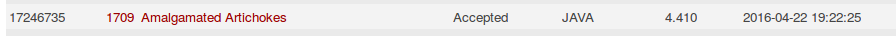
\includegraphics[width=\textwidth]{ProblemA}
\subsection{Problem D}
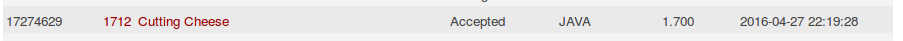
\includegraphics[width=\textwidth]{ProblemD}
\newpage

%%%%%%% start Problem A %%%%%%%%%%%%%%%%%%%%%%%%%%%%%%%%%%%%%%%%%%%

\section{Problem A: Amalgamated Artichokes}
\noindent \textbf{Results:} \\

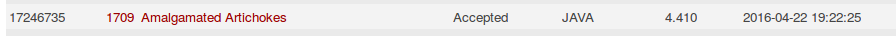
\includegraphics[width=\textwidth]{ProblemA} \\

\noindent \textbf{Background:} \\
~\indent Fatima Cynara is an analyst at Amalgamated Artichokes (AA). As with any company, AA has had some
very good times as well as some bad ones. Fatima does trending analysis of the stock prices for AA, and she
wants to determine the largest decline in stock prices over various time spans. For example, if over a span
of time the stock prices were 19, 12, 13, 11, 20 and 14, then the largest decline would be 8 between the first
and fourth price. If the last price had been 10 instead of 14, then the largest decline would have been 10
between the last two prices. \\
\indent Fatima has done some previous analyses and has found that the stock price over any period of time can
be modelled reasonably accurately with the following equation:
\begin{center}$price(x) = p \cdot (sin(a\cdot x + b) + cos(c\cdot x + d) + 2)$\end{center}
where $p,a,b,c,\ and\ d$ are constants.Fatima would like you to write a program to determine the largest
price decline over a given sequence of prices. You have to consider the prices only for integer values of $x$. \\

\noindent \textbf{Input:} \\
~\indent The input file contains several test cases. Each test case is on a single line containing 6 integers,
$p\ (1 \leq p \leq 1000),\ a,\ b,\ c,\ d\ (0 \leq a,b,c,d \leq 1000),\ and\ n\ (1 \leq n \leq 10^6)$. The first
5 integers are described above. The sequence of stock prices to consider are $price(1), price(2),..., price(n).$ \\

\noindent \textbf{Output:} \\
~\indent For each test case, display the maximum decline in stock prices. If there is no decline, display the
number '0'. Your output should have an absolute or relative error of at most $10^{-6}$. \\

\noindent \textbf{Sample Input:} \\
42 1 23 4 8 10  \\
100 7 615 998 801 3  \\
100 432 406 867 60 1000  \\

\noindent \textbf{Sample Output:} \\
104.855110477  \\
0.00           \\
399.303813

%%%%%%% end Problem %%%%%%%%%%%%%%%%%%%%%%%%%%%%%%%%%%%%%%%%%%%%%%%

\newpage

%%%%%%% Mathematical Formulation %%%%%%%%%%%%%%%%%%%%%%%%%%%%%%%%%%
\subsection{Mathematical Formulation}
Given an input of integers $p, a, b, c, d,\ and\ n$, the formula
$f(x) = p\cdot (sin(a\cdot x + b) + cos(c\cdot x + d) + 2)$ where $x \in [1, n]$, determine the largest
decrease between the integer values $x_i, x_j$ where $i \textless j$ and $x_i \geq x_j$ and there does
not exist another pair $x_k, x_l$ where $k \textless l$ and $x_k \geq x_l$ but $x_k - x_l \textgreater x_i - x_j$.

%%%%%%% Algorithm %%%%%%%%%%%%%%%%%%%%%%%%%%%%%%%%%%%%%%%%%%%%%%%%%

\subsection{Solution}
The main functionality of this algorithm is to plug in each point keeping track of the highest seen point, $h$,
the lowest seen point occuring after $l$, and the largest difference, $d = h-l$. It should be noted that since
we are always taking the difference between the two values, we can factor out the $\cdot p$ as well as neglect
the +2 portions of the formula. Also, to cut down on run time, it works in the java system if you \% pi each of
the entries before putting them into the sine and cosine functions. For whatever reason the larger the input,
the more costly the operation is.

\begin{algorithm}[H]
\caption{Main}
\begin{algorithmic}
    \Procedure{f}{x}
        \State $ab \gets$ (a*x+b) \% pi,
        \State $cd \gets$ (c*x+d) \% pi;
        \State return (Math.sin(ab) + Math.cos(cd))
    \EndProcedure
    \Procedure{Solve}{p, a, b, c, d, n}
        \State $val, h, l \gets$ f(1); $diff \gets$ 0
        \For{x $\in$ [2, n]} // if n = 1, do not execute
            \State $val \gets$ f(x)
            \If{$val \textgreater h$} // higher than current highest
                \State $h, l \gets$ val;
            \ElsIf{$val \textless l$} // lower than current lowest
                \State $l \gets$ val; $curDiff \gets$ h - l;
                \If{$curDiff \textgreater diff$}
                    $diff \gets$ curDiff;
                \EndIf
            \EndIf
        \EndFor
        \State \Call{print}{$p\cdot diff$}
    \EndProcedure
\end{algorithmic}
\end{algorithm}


%%%%%%% Correctness %%%%%%%%%%%%%%%%%%%%%%%%%%%%%%%%%%%%%%%%%%%%%%%

\subsection{Correctness}
%%%%%%% PROPOSITION 1 %%%%%%%%%%%%%%%
\begin{proposition}
~ \\ \indent We will determine the value of largest price decline over the interval $[1, n]$,
only considering $f(1), f(2),..., f(n)$.
\end{proposition}

\begin{proof}
~ \\ \indent We do this by keeping track of the largest price decline seen thus far, $diff$,
the current highest point seen, $h = f(x_i)$, and the current lowest point seen, $l = f(x_j)$,
such that $x_i \leq x_j,\ and\ f(x_i) \geq f(x_j)$. Therefore whenever we see a higher point,
$f(x_k) \textgreater f(x_i), x_k \textgreater x_i$, we update our $h = f(x_k)$ and reset our
lowest point to be $l = h$ since we are searching for the largest decline $\implies l$ must
occur \underline{after} $h$. Now every time that we see a number $f(x_m) \leq l$, we update
$l$ and check to see if our $h - l \geq diff$, if so we update diff, else we continue to the
next point.  If we see a higher point than $h$ we will repeat this process. Therefore we will
be looking at each subsequent highest correspoing following lowest points $\implies$ we will
see this largest price decline.
\end{proof}


%%%%%%% Analysis %%%%%%%%%%%%%%%%%%%%%%%%%%%%%%%%%%%%%%%%%%%%%%%%%%
\subsection{Analysis}

%%%%%%% PROPOSITION 1 %%%%%%%%%%%%%%%
\begin{proposition}
\label{numq}
The \underline{space complexity} of this algorithm is \textbf{O(1)}
\end{proposition}

\begin{proof}
~ \\ \indent This is due to the fact that we will only store the values $p, a, b, c, d, n, and diff$
as integer variables O(1):
\begin{center}
    Giving us a space complexity of \textbf{O(1)}
\end{center}
\end{proof}

%%%%%%% PROPOSITION 2 %%%%%%%%%%%%%%%
\begin{proposition}
\label{numq}
The \underline{time complexity} of this algorithm is \textbf{O(N)}
\end{proposition}

\begin{proof}
This is the case because our algorithm goes through the points $1, 2, ..., n$ once and only
calculates each value one time.
\begin{center}
    Giving us a time complexity of \textbf{O(N)}
\end{center}
\end{proof}

%%%%%%% Example %%%%%%%%%%%%%%%%%%%%%%%%%%%%%%%%%%%%%%%%%%%%%%%%%%%

\subsection{An Example}
Given the input of: \underline{42 1 23 4 8 10}, we will read this in as
$p = 42, a = 1, b = 23, c = 4, d = 8, and\ n = 10$. Then we will initialize our $h = l = f(1)$ and $diff = 0$.
Then starting with the second point until the 10th we will read through and record the values of what h, l, curDiff,
and diff are:

\begin{table}[H]
	\centering
	\resizebox{\textwidth}{!}{
	\begin{tabular}{c||c|c|c|c|c|c|c|c|c|c|}
		\toprule
		x =      & 1        & 2         & 3         & 4         & 5         & 6         & 7         & 8         & 9         & 10        \\
		\midrule
		f(x)    & -0.061724 & -1.090011 & 1.170641  & 1.380555  & -0.691700 & 0.170589  & -1.115995 & -1.070976 & 1.551270  & 0.359768 \\
        h       & -0.061724 & -0.061724 & 1.170641  & 1.380555  & 1.380555  & 1.380555  & 1.380555  & 1.380555  & 1.551270  & 1.551270 \\
        l       & -0.061724 & -1.090011 & 1.170641  & 1.380555  & -0.691700 & -0.691700 & -1.115995 & -1.115995 & 1.551270  & 0.359768 \\
        curDiff & --        & 1.028286  & --        & --        & 2.072255  & --        & 2.496550  & --        & --        & 1.191502 \\
        diff    & 0         & 1.028286  & 1.028286  & 1.028286  & 2.072255  & 2.072255  & 2.496550  & 2.496550  & 2.496550  & 2.496550 \\
        \bottomrule
	\end{tabular}}
\end{table}

Now multiplying our $diff$ by $p \implies 2.496550 \cdot 42 = 104.855110$ which is our solution.
%%%%%%% end Problem A %%%%%%%%%%%%%%%%%%%%%%%%%%%%%%%%%%%%%%%%%%%%%


%%%%%%% end Solution %%%%%%%%%%%%%%%%%%%%%%%%%%%%%%%%%%%%%%%%%%%%%%

\end{document}